\chapter{Introduzione}
		In questo capitolo si farà un'introduzione sull'importanza della voce, ponendo attenzione su cosa si intende per voice conversion e su cosa può comportare lo sviluppo di tali tecniche. Verrà inoltre analizzato lo stato dell'arte e descritto cosa si andrà a realizzare nell'ambito di questa tesi.
	
		\section{Ambito e scopo dell'applicazione}
			La voce è uno strumento comunicativo di cruciale importanza nelle relazioni umane in quanto ci consente di esprimere pensieri e di condividere informazioni con altri individui. Tuttavia essa non è unicamente informazione verbale, infatti oltre ad essere un veicolo per il contenuto linguistico che vogliamo esprimere è caratterizzata anche da aspetti acustici, come timbrica e intonazione.
			Queste ultime sono fondamentali poiché ci permettono di distinguere l’identità a cui corrisponde una determinata voce, tema che anch'esso ha sollevato recentemente molto interesse nel campo della ricerca sulla \textit{speaker recognition}\cite{speaker-recognition}.
			
			Con il termine \textit{voice conversion} si fa riferimento a tutte quelle tecniche che permettono di trasformare la voce di una persona \textit{sorgente} in un’altra voce \textit{target} preservando il contenuto linguistico, ovvero andando a modificare unicamente le caratteristiche dipendenti dall'interlocutore (come formanti, frequenza fondamentale, intonazione, intensità e durata) mantenendo invece quelle indipendenti che rappresentano il contenuto effettivo.
			
			La procedura tipica di VC si può riassumere in tre fasi fondamentali (Fig. \ref{fig:vc-pipeline})\cite{voice-conversion-overview}:
			\begin{enumerate}
				\item \textbf{Analisi}: Si ottiene una rappresentazione intermedia del segnale originale che sia più facilmente manipolabile o che renda più semplice l'estrazione di feature.
				\item \textbf{Trasformazione}: Si crea una mappatura tra le caratteristiche del segnale sorgente e quelle del segnale target e lo si trasforma.
				\item \textbf{Ricostruzione}: Si inverte la rappresentazione intermedia, a cui è stata applicata la trasformazione, al fine di ottenere il risultato finale come audio riproducibile.
			\end{enumerate}
			Risulta interessante notare come la VC non sia esclusivamente l'applicazione di una trasformazione ad un segnale ma includa anche delle rappresentazioni intermedie, il cui ruolo è cruciale in quanto potrebbero facilitare le operazioni di mappatura oppure causare artefatti e comprometterne il risultato.
			\begin{figure}%[h]
				\centering
				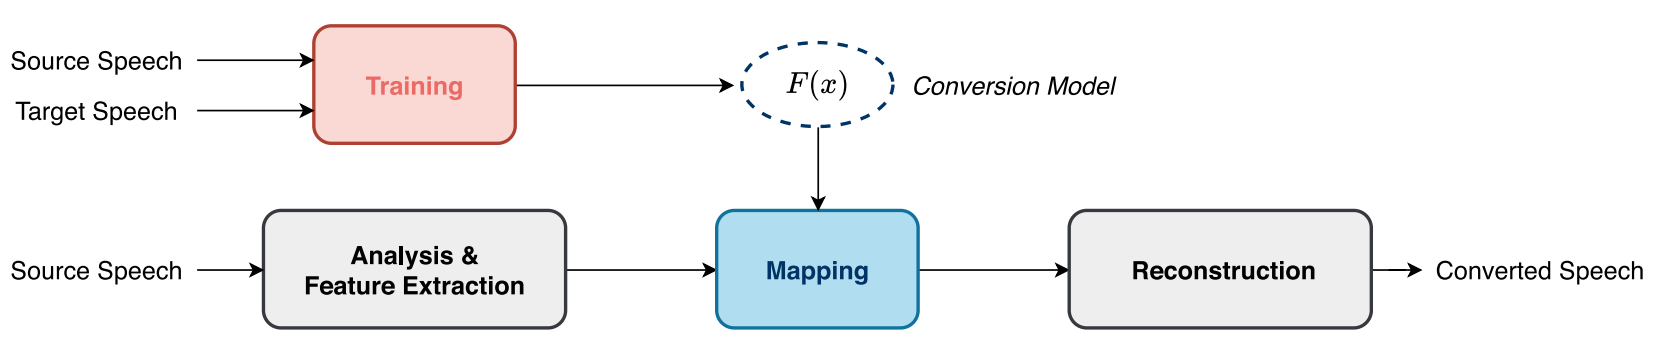
\includegraphics[width=1\linewidth]{figures/vc-pipeline}
				\caption{Pipeline tipica della voice conversion. Fonte \cite{voice-conversion-overview}.}
				\label{fig:vc-pipeline}
			\end{figure}
			L’interesse per la VC è dato dall’applicazione in vari campi come: sintesi vocale personalizzata, anonimizzazione voce e mimica vocale.
			Il tema è oggetto di ricerca nel campo della sintesi vocale e recentemente, grazie all’impiego di tecniche di deep learning, sono stati ottenuti importanti progressi. 
	
		\section{Stato dell'arte}
			In questa sezione si riporta una classificazione dei metodi per la voice conversion che impiegano tecniche di deep learning, estratta dall'analisi svolta da Sisman et al.\cite{voice-conversion-overview}, distinguendo in due categorie differenti in base alla tipologia del dataset impiegato nella fase di training: impiego di dati paralleli e impiego di dati non paralleli.
			
			\subsection{Dati paralleli}
			I primi studi si sono focalizzati sull'impiego di dati paralleli, vale a dire impiegando dataset formati da audio di parole, o frasi, pronunciati da entrambi gli speaker dei quali si vuole la conversione. Il task è piuttosto semplice poiché avendo a disposizione audio corrispondenti e allineati, il problema si riduce a creare una mappatura tra questi.
			
			Tuttavia ciò può risultare complesso e sebbene il problema dell'allineamento degli audio possa essere ovviato mediante l'impiego di encoder-decoder con meccanismo di attention\cite{attention-mechanism}, rimane comunque la problematica di avere a disposizione tali dati.
			
			\subsection{Dati non paralleli}
			Studi recenti hanno mostrato come siano possibili conversioni di voci anche con dati non paralleli, ovvero impiegando dataset che non presentano alcun audio di parole, o frasi, pronunciati da entrambi gli speaker di cui si vuole la conversione.
			
			In base all'approccio usato per realizzare ciò si possono distinguere quattro categorie principali:
			\begin{enumerate}
				\item Dati non paralleli di una coppia di speaker definita
				\item Impiego di sistemi Text-to-Speech
				\item Impiego di sistemi di Automated Speech Recognition
				\item Separazione del contenuto linguistico dallo speaker
			\end{enumerate}
			Si procede dunque con un'analisi di quelle che sono le tecniche allo stato dell'arte per ciascuno di essi.
			
			\paragraph{1) Dati non paralleli di una coppia di speaker definita}
			Le tecniche attualmente impiegate per la voice conversion con dati non paralleli di una coppia di speaker definita sono le stesse impiegate nell'\textit{image-to-image translation}, il cui obiettivo è trovare una mappatura da un dominio $X$ ad un dominio $Y$ mantenendone la struttura.
			Infatti come nella image translation si può volere, ad esempio, convertire fotografie di paesaggi in quadri di Monet, mantenendone il contesto originale rappresentato, così nella conversione di voci si vuole trasformare la voce tra due speaker differenti mantenendone il contenuto linguistico.
			
			Allo stato dell'arte abbiamo la CycleGAN-VC\cite{CycleGAN2017} proposta da Kaneko et al., in particolare con le sue varianti CycleGAN-VC2\cite{CycleGAN-VC2}, CycleGAN-VC3\cite{CycleGAN-VC3} e MaskCycleGAN-VC\cite{MaskCyclegan-VC} che verranno approfondite nel \autoref{chap:deep-learning}.
			
			\paragraph{2) Impiego di sistemi Text-to-Speech}
			Uno degli aspetti importanti della voice conversion è preservare il contenuto linguistico dalla voce sorgente a quella di destinazione, la quale è una caratteristica in comune con i sistemi Text-to-Speech (TTS) capaci di generare audio sintetico partendo da trascrizioni date. Questi ultimi si basano principalmente su modelli encoder-decoder e pertanto risulta possibile sfruttarli per la conversione attraverso tecniche di transfer learning\cite{transfer-learning-tts-vc}, condividendo la parte del decoder. Tuttavia la maggior parte di questi approcci richiede molti dati per la fase di addestramento del modello di TTS che non sempre sono disponibili.
			
			\paragraph{3) Impiego di sistemi Automated Speech Recognition}
			Gli approcci basati sul deep learning per la voice conversion richiedono grandi quantità di dati al fine di poter creare una rappresentazione latente che descriva il sistema fonetico.
			
			Tuttavia sappiamo che la maggior parte dei sistemi di riconoscimento automatico del parlato (ASR) sono già stati addestrati su grandi dati e descrivono correttamente il sistema fonetico, pertanto risulta interessante sfruttare la rappresentazione latente di essi nella conversione di voci.
			
			Un approccio particolarmente di successo consiste nel costruire un modello che sfrutti i phonetic posteriogram (PPG) estratti da un sistema di SI-ASR (speaker-independent ASR) al fine di creare una mappatura verso una voce target\cite{ppg-vc}.
			
			\paragraph{4) Separazione del contenuto linguistico dallo speaker}
			Per separare il contenuto linguistico dallo speaker sono possibili vari approcci, tra i più efficaci si menzionano l'impiego di instance normalization\cite{instance-normalization}, vector quantization\cite{vector-quantization} e l'utilizzo di auto-encoder\cite{auto-encoder}.
			
			Un auto-encoder impara a riprodurre l'output come il suo input, e per tale scopo deve costruire una rappresentazione latente intermedia. Questa codifica interna può essere vista come una forma compressa dell'input che mantiene tutte le informazioni necessarie per ricostruire il segnale originale in output.
			Questi approcci tuttavia tendono a generare audio di bassa qualità per via dell'eccessiva rimozione di informazione.
	
		\section{Contributo}
			Questo lavoro ha lo scopo di esplorare la conversione di voci con riduzione dello spettro sonoro. Partendo dall'idea per cui è possibile da un audio di una voce disaccoppiare la componente linguistica (indipendente dallo speaker) da quella acustica (dipendente dallo speaker), si vuole trovare una rappresentazione che riduca le caratteristiche di quest'ultima senza l'impiego di ulteriori dati o modelli pre-trained.
			
			Per fare ciò sono state impiegate tecniche tradizionali di speech processing per il pre-processamento dei dati, ottenendo così delle rappresentazioni in \textit{sine-wave speech}, \textit{buzz vocoded} e \textit{noise vocoded} degli stessi. Questi sono poi stati impiegati per addestrare un modello di tipo MaskCycleGAN-VC\cite{MaskCyclegan-VC}, stato dell'arte per quanto riguarda la voice conversion con dati non paralleli di coppie di speaker, e ne sono stati confrontati i risultati.
	